\documentclass[
  nojss]{jss}

%% recommended packages
\usepackage{orcidlink,thumbpdf,lmodern}

\usepackage[utf8]{inputenc}

\author{
Tomasz Woźniak~\orcidlink{0000-0003-2212-2378}\\University of Melbourne
}
\title{Fast and Efficient Bayesian Analysis of Structural Vector
Autoregressions Using the \proglang{R} package \pkg{bsvars} ~version
3.1}

\Plainauthor{Tomasz Woźniak}
\Plaintitle{Fast and Efficient Bayesian Analysis of Structural Vector
Autoregressions Using the R package bsvars}
\Shorttitle{\pkg{bsvars}: Bayesian Estimation of Structural Vector
Autoregressions}


\Abstract{
\noindent The \proglang{R} package \pkg{bsvars} provides a wide range of
tools for empirical macroeconomic and financial analyses using Bayesian
Structural Vector Autoregressions. It uses frontier econometric
techniques and compiled code written using \proglang{cpp} to ensure fast
and efficient estimation of these multivariate dynamic structural
models, possibly with many variables, complex identification strategies,
and non-linear characteristics. The models can be identified using
adjustable exclusion restrictions, heteroskedasticity, or non-normal
shocks and feature a flexible three-level equation-specific local-global
hierarchical prior distribution for the estimated level of shrinkage for
autoregressive and structural parameters. Additionally, the package
facilitates predictive and structural analyses such as impulse
responses, forecast error variance and historical decompositions,
forecasting, verification of heteroskedasticity and hypotheses on
autoregressive parameters, and analyses of structural shocks,
volatilities, and fitted values. These features differentiate
\pkg{bsvars} from existing \proglang{R} packages that either focus on a
specific structural model, do not consider heteroskedastic shocks, or
lack the implementation using compiled code.
}

\Keywords{Bayesian inference, Structural VARs, Gibbs sampler, exclusion
restrictions, heteroskedasticity, non-normal
shocks, forecasting, structural analysis, R}
\Plainkeywords{Bayesian inference, Structural VARs, Gibbs
sampler, exclusion restrictions, heteroskedasticity, non-normal
shocks, forecasting, structural analysis, R}

%% publication information
%% \Volume{50}
%% \Issue{9}
%% \Month{June}
%% \Year{2012}
%% \Submitdate{}
%% \Acceptdate{2012-06-04}

\Address{
    Tomasz Woźniak\\
    University of Melbourne\\
    Department of Economics\\
111 Barry Street\\
3053 Carlton, VIC, Australia\\
  E-mail: \email{tomasz.wozniak@unimelb.edu.au}\\
  URL: \url{https://github.com/donotdespair}\\~\\
  }


% tightlist command for lists without linebreak
\providecommand{\tightlist}{%
  \setlength{\itemsep}{0pt}\setlength{\parskip}{0pt}}




\usepackage[utf8]{inputenc} \usepackage{amsmath} \usepackage{natbib} \usepackage{booktabs}

\tolerance=1 \emergencystretch=\maxdimen \hyphenpenalty=10000
\hbadness=10000

\begin{document}



\begin{center}
\begin{tabular}{ l l}
Install the package: & \code{install.packages("bsvars")}\\
Load the package: & \code{library(bsvars)}\\[1ex]
CRAN repository: & \href{https://cran.r-project.org/package=bsvars}{cran.r-project.org/package=bsvars}\\
Website: & \href{https://bsvars.github.io/bsvars}{bsvars.github.io/bsvars}\\
Development repository: & \href{https://github.com/bsvars/bsvars}{github.com/bsvars/bsvars}\\
Suggestions and bug reporting: & \href{https://github.com/bsvars/bsvars/issues}{github.com/bsvars/bsvars/issues}\\
Discussions: & \href{https://github.com/bsvars/bsvars/discussions}{github.com/bsvars/bsvars/discussions}\\
Social media at Mastodon: & \href{https://fosstodon.org/@bsvars}{@bsvars@fosstodon.org}\\
Social media at Bluesky: & \href{https://bsky.app/profile/bsvars.bsky.social}{@bsvars.bsky.social}\\
email: & \href{mailto:bsvars@pm.me}{bsvars@pm.me}
\end{tabular}
\end{center}

\newpage
\section{Introduction}

Since the publication of the seminal paper by
\cite{sims1980macroeconomics} Structural Vector Autoregressions (SVARs)
have become benchmark models for empirical macroeconomic analyses.
Subsequently, they have found numerous applications in other fields and
are now indispensable in everyday work at central banks, treasury
departments and other economic governance institutions, as well as in
finance, insurance, banking, and economic consulting.

The great popularity of these multivariate dynamic structural models was
gained because they incorporate the reduced and structural forms into a
unified framework. On the one hand, they capture the essential
properties of macroeconomic and financial time series such as
persistence, dynamic effects, system modelling, and potentially
time-varying conditional variances. On the other hand, they control for
the structure of an economy, system, or market through the
contemporaneous effects and, thus, they identify contemporaneously and
temporarily uncorrelated shocks that can be interpreted structurally.
All these features make it possible to estimate the dynamic causal
effects of the shocks on the measurements of interest. These effects are
interpreted as the propagation of the well-isolated and unanticipated
cause -- a contemporaneously and temporarily independent shock -- within
the considered system of variables throughout the predictable future.

This flexibility comes at a cost of dealing with local identification of
the model, sharply growing dimension of the parameter space with the
increasing number of variables, and the estimation of latent variables.
Bayesian inference provides original solutions to each of these
challenges often deciding on the feasibility of the analyses with a
demanded model including many variables, conditional heteroskedasticity,
and sophisticated identification of the structural shocks. In this
context, Bayesian estimation using Markov Chain Monte Carlo methods
grants the certainty of reliable estimation of the parameters of
interest through the straightforward process of diagnosing the
algorithm's convergence but it might incur substantial computational
cost.

The paper at hand and the corresponding package \pkg{bsvars} by
\cite{bsvars} for \proglang{R} \citep{Rcore} provide tools for empirical
macroeconomic and financial analyses using Bayesian SVARs. It addresses
the considered challenges by choosing a convenient model formulation,
applying frontier econometric techniques, and relying on compiled code
written using \proglang{cpp} to ensure fast and efficient estimation.
Additionally, it offers a great flexibility in choosing the model
specification and identification pattern, modifying the prior
assumptions, and accessing interpretable tabulated or plotted outputs.

More specifically, the package uses the SVAR models featuring a standard
reduced form VAR equation following \cite{Banbura2010}
\citep[see also][]{Wozniak2016} and a structural equation linking the
reduced form error term to the structural shocks via the structural
matrix as in \cite{LSUW2024} and \cite{chankoopyu2024}. The normal prior
distribution for the autoregressive parameters implements the
interpretability of the Minnesota prior by \cite{Doan1984} by centring
it around the mean that reflects unit-root nonstationarity or
stationarity of the variables and a adjustable level of shrinkage
depending on the equation and exhibiting exponential decay with the
increasing autoregressive lag order. The prior distribution for the
structural matrix is generalised-normal by \cite{WaggonerZha2003} which
preserves the shape of the likelihood function
\citep[see][]{Wozniak2015}. Both of these priors are combined with the
flexible three-level equation-specific local-global hierarchical prior
distribution for the estimated level of shrinkage as in \cite{LSUW2024}
improving the model fit. The estimation of the level of shrinkage was
shown to substantially improve forecasting performance of VAR models by
\cite{Giannone2015}. Additionally, these specification choices lead to
an efficient equation-by-equation Gibbs sampler for the posterior
distribution of the autoregressive and structural parameters proposed by
\cite{chankoopyu2024} and \cite{WaggonerZha2003} respectively.

\begin{figure}
\centering

\includegraphics[width=2in,height=2.314in]{bsvars.png}
\caption{The hexagonal package logo features an impulse response that
can be fully reproduced using the \pkg{bsvars} package following a
script available at:
\href{https://github.com/donotdespair/naklejki/blob/master/bsvars/bsvars.R}{github.com/donotdespair/naklejki/blob/master/bsvars/bsvars.R}}
\end{figure}

All the structural models in the \pkg{bsvars} package can be identified
using highly adaptable exclusion restrictions proposed by
\cite{WaggonerZha2003} and use the structural matrix sign normalisation
by \cite{WaggonerZha2003norm}. However, one might also choose not to
impose any restrictions on the structural matrix and identify it through
heteroskedasticity following the ideas by \cite{Rigobon03} or by
non-normal shocks as proposed by \cite{Lanne2010}. Therefore, the
package offers a range of models for conditional variance including a
homoskedastic model with time-invariant variances. The list of
heteroskedastic specifications is opened by Stochastic Volatility (SV)
model in two versions: non-centred as in \cite{LSUW2024} and centred
used by \cite{chankoopyu2024}, and is followed by the Markov-switching
heteroskedasticity (MSH) model proposed by \cite{brunnermeier2021} with
the Bayesian implementations following \cite{Wozniak2015} in two
versions: with stationary Markov process and its sparse version that
facilitates the estimation of the number of states and non-parametric
interpretations. Similarly, a model with non-normal shocks is
implemented in two versions of the normal mixture (MIX) model: with a
finite number of components as in \cite{FruhwirthSchnatter2006} and in
its sparse representation serving as an approximation of a
non-parametric infinite mixture as proposed by \cite{malsiner2016model}.

The \proglang{R} package \pkg{bsvars} implements a wide range of tools
for structural and predictive analyses. The former encompass the methods
comprehensively revised by \citep[][Chapter 4: SVAR Tools]{KL2017} and
include the impulse response functions, forecast error variance
decompositions, historical decompositions, as well as the basic analysis
of fitted values, structural shocks, conditional standard deviations and
regime probabilities for MSH and MIX models. The predictive analysis
includes Bayesian forecasting implemented through an algorithm sampling
from the predictive density of the unknown future values of the
dependent variables. Methods \texttt{summary()} and \texttt{plot()}
support the user in the interpretations and visualisation of these types
of analyses.

A distinguishing feature of the package are the Bayesian model
diagnostic tools for the verification of heteroskedasticity and
hypotheses on autoregressive parameters using Savage-Dickey Density
Ratios (SDDRs) by \cite{Verdinelli1995}. The SDDRs represent the Bayes
factors for sharp hypotheses and are reliable, precisely estimated, and
straightforward to compute once the posterior sample is available. As
shown by \cite{LW2017} and \cite{LSUW2024}, SDDRs are a pragmatic tool
for the Bayesian assessment of a null hypothesis of homoskedasticity in
heteroskedastic models allowing to verify partial or global
identification through heteroskedasticity. A general implementation of
SDDRs for the autoregressive parameters facilitates verification of
restrictions on any conditional mean parameters of the model.

Multivariate dynamic modelling, both Bayesian and frequentist, has found
some traction in \proglang{R} in the recent years, which resulted in
many new packages available on the CRAN repository. The most relevant
developments in frequentist approach include the package \pkg{MTS} by
\cite{MTS} covering a wide range of benchmark models for multivariate
time series analysis in economics in finance. If it is about structural
models, then the seminal package \pkg{vars} by \cite{vars} covering
homoskedastic VAR and Vector Error Correction (VEC) models provides an
unmatched in its reliability teaching and basic analysis tool set.

Notable Bayesian implementations include two packages focusing on
specific models important from the point of view of historical
developments in the field, namely, the package \pkg{BVAR} by \cite{BVAR}
providing tools for the estimation and analysis proposed by
\cite{Giannone2015} and package \pkg{bvarsv} by \cite{bvarsv} focusing
on the heteroskedastic VAR proposed by \cite{Primiceri2005}. Other
packages that have been archived and are no longer available on CRAN are
the package \pkg{MSBVAR} by \cite{MSBVAR} focusing on the Markov
switching model by \cite{Sims2006} and package \pkg{VARsignR} by
\cite{VARsignR} provided a treatment of Bayesian SVARs identified via
sign restrictions by \cite{uhlig2005effects},
\cite{rubio2010structural}, and \cite{fry2011sign}. The package
\pkg{bvartools} by \cite{bvartools} provides some functionality focusing
on Bayesian inference of reduced form VAR and VEC models. Finally, the
package \pkg{shrinkTVP} by \cite{shrinkTVP} implementing heteroskedastic
time-varying parameters regression model with shrinkage on the state
space as proposed by \cite{Bitto2019} and \cite{Cadonna2020} gives a
possibility of estimating an SVAR model as well.

However, the most relevant package to compare \pkg{bsvars} to is the
package \pkg{svars} by \cite{svars} focusing on frequentist inference
for SVAR models identified via exclusion restrictions,
heteroskedasticity, and non-normal shocks and implementing a range of
models that are feasible to estimate using the maximum likelihood
method. The similarity to the functionality of package \pkg{bsvars}
include the selection of models, such as the MSH and with non-normal
residuals, as well as the selection of tools for structural analyses
including impulse responses, historical and forecast error variance
decompositions. However, the package \pkg{svars} implements maximum
likelihood and bootstrap procedures for the analysis of the model
parameters and offers some specification testing procedures.

In this context, the \pkg{bsvars} package implements a range of novel
solutions and models for Bayesian analysis. One differentiating example
is the implementation of the SVAR models with Stochastic Volatility that
is not covered by the package \pkg{svars}. This model is particularly
important in the context of the recent literature clearly indicating
that the single extension of VARs leading to marginally largest
improvements in the model fit or forecasting performance is the
extension by the Stochastic Volatility as shown e.g.~by
\cite{Clark2015}, \cite{Chan2018}, \cite{carriero_large_2019},
\cite{chan2020large}, and \cite{bertsche2022identification}. Another
such example are sparse MSH and MIX models based on the hierarchical
prior distribution proposed by \cite{malsiner2016model}, which decides
on the infeasibility of their frequentist implementation. Additionally,
the package \pkg{bsvars} benefits from the advantage of Bayesian
approach that facilitates the estimation for models with potentially
many variables, autoregressive lags inflating the dimension of
parameters space relative to the number of observations in
macroeconomics datasets, Markov-switching regimes or normal mixture
components, all of which are the factors constraining the feasibility of
maximum likelihood approaches. Finally, the model specification,
application of econometric advances and compiled code makes the
estimation in package \pkg{bsvars} much faster than the implementations
in packages \pkg{bvarsv} and \pkg{MSBVAR}.

\section{Bayesian Analysis of Structural VARs}\label{sec:bayes}

This section scrutinises the modelling framework used in the package
focusing on the specification of the models, prior distributions,
hypotheses verification tools, and estimation. The reader is referred to
\citep[][Chapter 4: SVAR Tools]{KL2017} for the exposition of the
standard tools for the analysis of SVAR models, such as the impulse
responses, and historical and forecast error variance decompositions, as
their implementation in the package closely follows this resource.

\subsection{Structural VARs}\label{ssec:svars}

All of the models in the package \pkg{bsvars} share the reduced and
structural form equations, as well as the hierarchical prior
distributions for these parameters following \cite{LSUW2024}. The
reduced form equation is the VAR equation with \(p\) lags specified for
an \(N\)-vector \(\mathbf{y}_t\) collecting observations on \(N\)
variables at time \(t\): \begin{align}
\mathbf{y}_t &= \mathbf{A}_1 \mathbf{y}_{t-1} + \dots + \mathbf{A}_p \mathbf{y}_{t-p} + \mathbf{A}_d \mathbf{d}_t +  \boldsymbol{\varepsilon}_t, \label{eq:var}
\end{align} where \(\mathbf{A}_i\) are \(N\times N\) matrices of
autoregressive slope parameters, \(\mathbf{d}_t\) is a \(D\)-vector of
deterministic terms, always including a constant term, and possibly
exogenous variables, \(\mathbf{A}_d\) is an \(N\times D\) matrix of the
corresponding parameters, and \(\boldsymbol{\varepsilon}_t\) collects
the \(N\) reduced form error terms. Collect all the autoregressive
matrices and the slope terms in an \(N\times (Np+D)\) matrix
\(\mathbf{A} = \begin{bmatrix}\mathbf{A}_1& \dots & \mathbf{A}_p & \mathbf{A}_d\end{bmatrix}\)
and the explanatory variables in a \((Np+D)\)-vector
\(\mathbf{x} = \begin{bmatrix}\mathbf{y}_{t-1} & \dots & \mathbf{y}_{t-p} & \mathbf{d}_{t} \end{bmatrix}'\).
Then equation \eqref{eq:var} can be written in the matrix form as
\begin{align}
\mathbf{y}_t &= \mathbf{A}\mathbf{x}_t + \boldsymbol{\varepsilon}_t. \label{eq:rf}
\end{align} Each of the rows of the matrix \(\mathbf{A}\), denoted by
\([\mathbf{A}]_{n\cdot}\) follows a multivariate conditional normal
prior distribution, given the equation-specific shrinkage
hyper-parameter \(\gamma_{A.n}\), with the mean vector
\(\underline{\mathbf{m}}_{n.A}\) and the covariance
\(\gamma_{A.n}\underline{\Omega}_A\), denoted by: \begin{align}
[\mathbf{A}]_{n\cdot}'\mid\gamma_{A.n} \sim\mathcal{N}_{Np+1}\left( \underline{\mathbf{m}}_{n.A}, \gamma_{A.n}\underline{\Omega}_A \right),
\end{align} where \(\underline{\mathbf{m}}_{n.A}\) is specified in-line
with the Minnesota prior by \cite{Doan1984} as a vector of zeros if all
of the variables are unit-root stationary, or containing value 1 in its
\(n\textsuperscript{th}\) element if the \(n\textsuperscript{th}\)
variable is nonstationary. By default,
\(\underline{\boldsymbol{\Omega}}_A\) is a diagonal matrix with vector
\(\begin{bmatrix}\mathbf{p}^{-2\prime}\otimes\boldsymbol{\imath}_N' & 100\boldsymbol{\imath}_d'\end{bmatrix}'\)
on the main diagonal, where \(\mathbf{p}\) is a vector containing a
sequence of integers from 1 to \(p\) and \(\boldsymbol\imath_N\) is an
\(N\)-vector of ones. Both, \(\underline{\mathbf{m}}_{n.A}\) and
\(\underline{\boldsymbol{\Omega}}_A\) can be modified by the user. This
specification includes the shrinkage level exponentially decaying with
the increasing lag order, relatively large prior variances for the
deterministic term parameters, and the flexibility of the hierarchical
prior that leads to the estimation of the level of shrinkage as proposed
by \cite{Giannone2015}. The latter feature is facilitated by assuming a
3-level local-global hierarchical prior on the equation-specific reduced
form parameters shrinkage given by \begin{align}
\gamma_{A.n} | s_{A.n}  &\sim\mathcal{IG}2\left(s_{A.n}, \underline{\nu}_A\right),\\
s_{A.n} | s_{A} &\sim\mathcal{G}\left(s_{A}, \underline{a}_A\right),\\
s_{A} &\sim\mathcal{IG}2\left(\underline{s}_{s_A}, \underline{\nu}_{s_A}\right),
\end{align} where \(\mathcal{G}\) and \(\mathcal{IG}2\) are gamma and
inverted gamma 2 distributions \citep[see][Appendix A]{Bauwens1999},
hyper-parameters \(\gamma_{A.n}\), \(s_{A.n}\), and \(s_{A}\) are
estimated, and \(\underline{\nu}_A\), \(\underline{a}_A\),
\(\underline{s}_{s_A}\), and \(\underline{\nu}_{s_A}\) are all set by
default to value 10 to assure appropriate level of shrinkage towards the
prior mean. The values of the latter hyper-parameters can be modified by
the user.

The structural form equation determines the linear relationship between
the reduced-form innovations \(\boldsymbol{\varepsilon}_t\) and the
structural shocks \(\mathbf{u}_t\) using the \(N\times N\) structural
matrix \(\mathbf{B}_0\): \begin{align}
\mathbf{B}_0\boldsymbol{\varepsilon}_t = \mathbf{u}_t.\label{eq:sf}
\end{align} The structural matrix specifies the contemporaneous
relationship between the variables in the system and determines the
identification of the structural shocks from vector \(\mathbf{u}_t\).
Its appropriate construction may grant specific interpretation to one or
many of the shocks. The package \pkg{bsvars} facilitates the
identification of the structural matrix and the shocks via exclusion
restrictions \citep[see][Chapter 8]{KL2017} and/or through
heteroskedasticity or non-normal shocks \citep[][Chapter 14]{KL2017}.
The zero restrictions are imposed on the structural matrix row-by-row
following the framework proposed by \cite{WaggonerZha2003} via the
following decomposition of the \(n\textsuperscript{th}\) row of the
structural matrix, denoted by \([\mathbf{B}_0]_{n\cdot}\): \begin{align}
[\mathbf{B}_0]_{n\cdot} = \mathbf{b}_n\mathbf{V}_n, \label{eq:restrictions}
\end{align} where \(\mathbf{b}_n\) is a \(1\times r_n\) vector
collecting the elements to be estimated and the \(r_n\times N\) matrix
\(\mathbf{V}_n\) including zeros and ones placing the estimated elements
in the demanded elements of \([\mathbf{B}_0]_{n\cdot}\).

The structural matrix \(\mathbf{B}_0\) follows a conditional
generalised-normal prior distribution by \cite{WaggonerZha2003} recently
revised by \cite{Arias2018} that is proportional to: \begin{align}
\mathbf{B}_0\mid\gamma_{B.1},\dots,\gamma_{B.N} \sim |\det(\mathbf{B}_0)|^{\underline{\nu}_B - N} \exp\left\{-\frac{1}{2} \sum_{n=1}^{N} \gamma_{B.n}^{-1} \mathbf{b}_n\mathbf{b}_n' \right\},
\end{align} with the shape parameter \(\underline{\nu}_B \geq N\) and
the equation-specific structural parameter shrinkage \(\gamma_{B.n}\).
The default value of the shape parameter \(\underline{\nu}_B\) set to
\(N\) makes this prior a conditional, zero-mean \(r_n\)-variate normal
prior distribution for \(\mathbf{b}_n\) with the diagonal covariance and
the diagonal element \(\gamma_{B.n}\). The shape parameter can be
modified by the user though.

This prior specification is complemented by a 3-level local-global
hierarchical prior on the equation-specific structural parameters
shrinkage given by \begin{align}
\gamma_{B.n} | s_{B.n}  &\sim\mathcal{IG}2\left(s_{B.n}, \underline{\nu}_b\right),\\
s_{B.n} | s_{B} &\sim\mathcal{G}\left(s_{B}, \underline{a}_B\right),\\
s_{B} &\sim\mathcal{IG}2\left(\underline{s}_{s_B}, \underline{\nu}_{s_B}\right),
\end{align} where hyper-parameters \(\gamma_{B.n}\), \(s_{B.n}\), and
\(s_{B}\) are estimated and \(\underline{\nu}_b\), \(\underline{a}_B\),
\(\underline{s}_{s_B}\), and \(\underline{\nu}_{s_B}\) are fixed to
values 10, 10, 1, and 100 respectively to assure a flexible dispersed
distribution \emph{a priori} but they can be modified by the user.

Finally, all of the models share the zero-mean conditional normality of
the structural shocks given the past observations with the diagonal
covariance matrix with the \(N\)-vector of structural shocks' variances,
\(\boldsymbol{\sigma}_t^2\), on the main diagonal: \begin{align}
\mathbf{u}_t\mid\mathbf{x}_t \sim\mathcal{N}_{N}\left( \mathbf{0}_N, \text{diag}\left(\boldsymbol{\sigma}_t^2\right) \right).
\end{align} The diagonal covariance matrix, together with the joint
normality, implies contemporaneous independence of the structural shocks
which is the essential feature allowing for the estimation of dynamic
effects to a well-isolated cause that is not influenced by other factors
in the SVAR models.

The model parts described in the current section are common to all the
models considered in the package \pkg{bsvars}. The alternative model
specifications are distinguished by the characterisation of the
conditional variances collected in vector \(\boldsymbol{\sigma}_t^2\).

\subsection{Models for Conditional Variances}\label{ssec:variances}

The \pkg{bsvars} package offers five alternative specifications for the
conditional variance process.

\subsubsection{Homoskedastic model}

The first such specification is a homoskedastic model for which the
conditional variance of every shock is equal to \begin{align}
\sigma_{n.t}^2 = 1 \label{eq:homosk}
\end{align} for all \(t\). This setup results in a simple SVAR model
that is quick to estimate. Note that in this model the conditional
covariance of the data vector, \(\mathbf{y}_t\) is equal to
\((\mathbf{B}_0'\mathbf{B}_0)^{-1}\). The point at which this model is
standardized as in equation \eqref{eq:homosk} is the benchmark value for
the all other heteroskedastic models whose conditional variances hover
around value 1.

\subsubsection{Stochastic Volatility}

The heteroskedastic model with Stochastic Volatility is implemented in
two versions: non-centred by \cite{LSUW2024} and centred
\cite{chankoopyu2024}. In these models, the conditional variances for
each of the shocks are given by \begin{align}
\text{non-centred:}&&\sigma_{n.t}^2 &= \exp\left\{\omega_n h_{n.t}\right\}\\
\text{centred:}&&\sigma_{n.t}^2 &= \exp\left\{\tilde{h}_{n.t}\right\},
\end{align} where the parameter \(\omega_n\) denotes the plus-minus
square root of the conditional variance for the log-conditional variance
process and will be referred to as the
\emph{volatility of the log-volatility}, whereas \(h_{n.t}\) and
\(\tilde{h}_{n.t}\) are the log-volatility processes following an
autoregressive equation \begin{align}
\text{non-centred:}&&h_{n.t} &= \rho_n h_{n.t-1} + v_{n.t}, && v_{n.t}\sim\mathcal{N}\left(0,1\right)\\
\text{centred:}&&\tilde{h}_{n.t} &= \rho_n \tilde{h}_{n.t-1} + \tilde{v}_{n.t}, && \tilde{v}_{n.t}\sim\mathcal{N}\left(0,\sigma_v^2\right)
\end{align} with the initial values \(h_{n.0} = \tilde{h}_{n.0} = 0\),
where \(\rho_n\) is the autoregressive parameter, \(v_{n.t}\) and
\(\tilde{v}_{n.t}\) are the Stochastic Volatility normal innovations,
and \(\sigma_v^2\) is the conditional variance of \(\tilde{h}_{n.t}\) in
the centred parameterisation.

\begin{CodeChunk}
\begin{figure}

{\centering 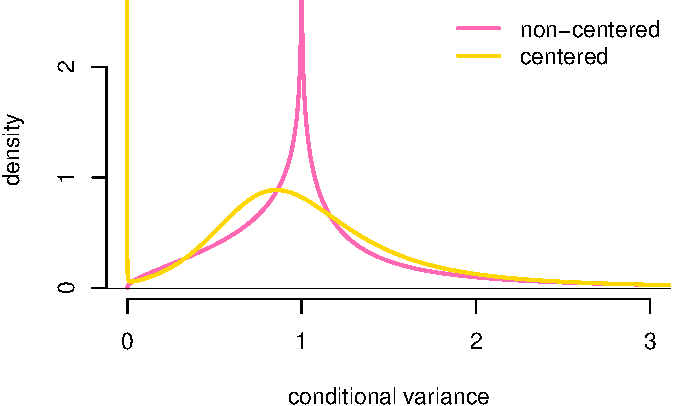
\includegraphics{bsvars_files/figure-latex/plot_cv_prior-1} 

}

\caption[Marginal prior density of a structural shock conditional variance in the two SV models]{Marginal prior density of a structural shock conditional variance in the two SV models. Sourse: Lütkepohl et al. (2024).}\label{fig:plot_cv_prior}
\end{figure}
\end{CodeChunk}

The priors for these models include a uniform distribution for the
autoregressive parameter \begin{align}
\rho_n \sim\mathcal{U}(-1,1),
\end{align} which assures the stationarity of the log-volatility process
and sets its unconditional expected value to
\(E[h_{n.t}] = E[\tilde{h}_{n.t}] =0\). The prior distribution for the
volatility of the log-volatility parameter in the non-centred and the
conditional variance of the log-volatility in the centred
parameterisation follow a multi-level hierarchical structures given by:
\begin{align}
\text{non-centred:}&&\omega_n\mid \sigma_{\omega.n}^2 &\sim\mathcal{N}\left(0, \sigma_{\omega.n}^2\right),\qquad
\sigma_{\omega.n}^2 \mid s_\sigma\sim\mathcal{G}(s_\sigma, \underline{a}_\sigma), \qquad
s_\sigma \sim\mathcal{IG}2(\underline{s}, \underline{\nu})\\
\text{centred:}&&\sigma_v^2 \mid s_v &\sim\mathcal{IG}2(s_v, \underline{a}_v), \qquad
s_v \mid s_\sigma\sim\mathcal{G}(s_\sigma, \underline{a}_\sigma), \qquad
s_\sigma \sim\mathcal{IG}2(\underline{s}, \underline{\nu})
\end{align} where parameters \(\sigma_{\omega.n}^2\) and \(s_v\) follow
gamma distribution with expected value equal to
\(s_\sigma\underline{a}_\sigma\). In this hierarchical structure the
hyper-parameters \(\omega_n\), \(\sigma_{\omega.n}^2\), \(\sigma_v^2\),
\(s_v\), and \(s_\sigma\) are estimated, while \(\underline{a}_v\),
\(\underline{a}_\sigma\), \(\underline{\nu}\), and \(\underline{s}\) are
set to values 1, 1, 1, and 0.1, respectively, by default and can be
modified by the user.

Both of the SV models share a number of features, such as the
flexibility of hierarchical priors with estimated hyper-parameters
granting better fit to data and improved forecasting performance, and
they facilitate the identification of the structural matrix
\(\mathbf{B}_0\) and shocks through heteroskedasticity following the
original ideas by \cite{bertsche2022identification} and
\cite{lewis_identifying_2021}. However, they differ with respect to the
features analysed by \cite{LSUW2024} that are presented in Figure
\ref{fig:plot_cv_prior} plotting the marginal prior distribution of the
conditional variances, \(\sigma_{n.t}^2\), in the two SV models. These
densities are implied by the SV model specifications presented in this
section. The centred parameterisation concentrate the prior probability
mass around point 1 only mildly and goes to infinity when the
conditional variance goes to zero. The non-centred parameterisation, on
the other hand, concentrates the prior probability mass around point 1
more strongly, goes to zero when the conditional variance goes to zero,
and features fat right tail. Finally, in the non-centred
parameterisation homoskedasticity can be verified by testing the
restriction \(\omega_n = 0\) \citep[see][]{LSUW2024}.

\subsubsection{Markov-switching heteroskdasticity}

In another heteroskedastic model, the MSH one, the time-variation of the
conditional variances is determined by a discrete-valued Markov process
\(s_t\) with \(M\) regimes: \begin{align}
\sigma_{n.t}^2 = \sigma_{n.s_t}^2.
\end{align} All of the variances switch their values at once according
to the latent Markov process takes the values
\(s_t = m\in\{1,\dots,M\}\). The properties of the Markov process itself
are determined by the transition matrix \(\mathbf{P}\) whose
\([\mathbf{P}]_{i.j}\) element denotes the transition probability from
regime \(i\) to regime \(j\) over the next period. The process' initial
probabilities are estimated and denoted by the \(M\)-vector
\(\boldsymbol{\pi}_0\). In this model proposed by
\cite{brunnermeier2021}, the variances in the \(n\textsuperscript{th}\)
equation sum to \(M\), each of them has the prior expected value equal
to 1, and their regimes are given equal prior probabilities of
occurrence equal to \(M^{-1}\). Therefore, the prior for the conditional
variances is the \(M\)-variate Dirichlet distribution: \begin{align}
M^{-1}\left(\sigma_{n.1}^2, \dots, \sigma_{n.M}^2\right) \sim\mathcal{D}irichlet_M(\underline{e}_\sigma, \dots, \underline{e}_\sigma), \label{eq:sigmaMSprior}
\end{align} where the hyper-parameter \(\underline{e}_\sigma = 1\) is
fixed. Each of the rows of the transition matrix as well as the initial
state probabilities follow the Dirichlet distribution as well:
\begin{align}
[\mathbf{P}]_{m\cdot} \sim\mathcal{D}irichlet_M(\underline{e}, \dots, \underline{e})\quad\text{and}\quad \boldsymbol{\pi}_0 \sim\mathcal{D}irichlet_M(\underline{e}_0, \dots, \underline{e}_0).
\end{align}

The package \pkg{bsvars} offers two alternative models based on MSH. The
first is characterised by a stationary Markov process with no absorbing
state, and with a positive minimum number of regime occurrences
following \cite{Wozniak2015}. In this model, the hyper-parameter
\(\underline{e} = \underline{e}_0\) is fixed to 1 by default and can be
modified by the user. The other model represents a novel proposal of a
sparse representation that fixes the number of regimes to an
over-fitting value \(M=20\) (or specified by the user). In this model,
many of the regimes will have zero occurrences throughout the sample,
which allows the number of regimes with non-zero occurrences to be
estimated following the ideas by \cite{malsiner2016model}. Its prior
specification is complemented by a hierarchical prior for the
hyper-parameter \(\underline{e}\): \begin{align}
\underline{e} \sim \mathcal{IG}2\left(\underline{s}_e, \underline{\nu}_e\right). \label{eq:sparseprior}
\end{align} In the sparse MSH model the regimes feature label switching,
which excludes regime-specific interpretation of parameters. Instead,
the estimated sequence of conditional variances, \(\sigma_{n.t}^2\),
enjoys standard interpretations. Furthermore, both MSH models provide
identification through heteroskedasticity following the ideas by
\cite{LLM2010} and \cite{LW2017}. The latter paper provides framework
for verifying the identification, which in the \pkg{bsvars} package is
implemented by verifying the homoskedasticity hypothesis represented by
the restriction \begin{align}
\sigma_{n.1}^2 = \dots = \sigma_{n.M}^2 = 1.\label{eq:homonorm}
\end{align}

\subsection{Models with Non-Normal Shocks}

Identification via non-normality of the structural shocks is implemented
in the package using the mixture of normal component model (MIX)
following the proposal by \cite{Wozniak2015}. In this model, the
structural shocks follow a conditional \(N\)-variate normal distribution
given the state variable \(s_t=m\in\{1,\dots,M\}\); \begin{align}
u_t\mid s_t=m \sim\mathcal{N}_N\left(\mathbf{0}_n, \boldsymbol{\sigma}_m^2 \right),
\end{align} and where the states are predicted to occur in the next
period with probability \(\pi\) which is an \(M\)-vector. Therefore,
unconditionally, the shocks follow a mixture of zero-mean normal
components with variance \(\boldsymbol{\sigma}_m^2\) for
\(m\in\{1,\dots,M\}\). The prior distribution for the conditional
variances is the same as for the MSH model and is given by equation
\eqref{eq:sigmaMSprior}. The predictive state probabilities follow a
Dirichlet distribution: \begin{align}
\boldsymbol{\pi} \sim\mathcal{D}irichlet_M(\underline{e}, \dots, \underline{e}).\label{eq:dirichletmix}
\end{align} Despite the predictive state probabilities being constant
the classification of the observations into the states is performed via
the estimated filtered probabilities \(\Pr[s_t=m\mid y_t]\)
\citep[see][for a recent review of the method]{song2021markov}.

The MIX model comes in two versions as well. The first is the finite
mixture model \citep[see e.g.][]{FruhwirthSchnatter2006} in which the
number of states, \(M\), is fixed and the state probabilities are
positive. The latter condition requires non-zero regime occurrences over
the sample, a condition that is imposed in the package implementation.
An alternative specification is referred to as the sparse mixture model
and is based on the proposal by \cite{malsiner2016model}. In this model,
the number of the finite mixture model's components is set to be larger
than the real number of the components. The number of components with
non-zero probability of occurrence is, therefore, estimated. This sparse
structure of normal components many of which are allowed to have zero
probability is implemented thanks to the prior specified for the
hyper-parameter \(\underline{e}\) of Dirichlet distribution as in
equation \eqref{eq:sparseprior}.

The MIX models facilitate the identification through non-normality as
proposed by \cite{Lanne2010}. The hypothesis of normality contradicting
the identification is verified by checking whether restriction as in
equation \eqref{eq:homonorm} holds.

\subsection{Model diagnostics using SDDRs}

\cite{Verdinelli1995}

\subsubsection{Verifying heteroskedasticity}

\subsubsection{Verifying autoregressive specification}

\subsection{Posterior Samplers and Computational Details}\label{sec:posterior}

In this section we explain the the \pkg{bsvars} package implementation
of fast and efficient estimation algorithms obtained thanks to the
application of appropriate model specification and frontier econometric
techniques best described in \cite{LSUW2024} and \cite{Wozniak2015}, and
compiled code written in \proglang{cpp}.

The objective for choosing the model equations and the prior
distributions was to make the estimation using Gibbs sampler technique
\citep[see e.g.][]{CasellaGeorge1992} and well-specified
easy-to-sample-from full conditional posterior distributions. Therefore,
the package relies on the reduced form equation \eqref{eq:rf} for the
VAR model. This choice is fairly uncommon in the SVAR literature but it
simplifies the estimation of the autoregressive parameters
\(\mathbf{A}\) directly in the form as they are used for the
computations of impulse responses or forecast error variance
decomposition. This choice combined with the specification of the
structural form equation \eqref{eq:sf} facilitates the application of
the row-by-row sampler by \cite{chankoopyu2024}. As shown by
\cite{carriero_large_2019}, relative to the joint estimation of the
matrix \(\mathbf{A}\) in one step, a usual practice in reduced form
VARs, the row-by-row estimation in SVARs can reduce computational
complexity of Bayesian estimation from \(\mathcal{O}(N^6)\) to
\(\mathcal{O}(N^4)\).

The estimation of the structural form equation \eqref{eq:sf} is
implemented following the quickly converging, efficient, and providing
excellent mixing sampling algorithm by \cite{WaggonerZha2003}. It offers
a flexible framework for setting exclusion restrictions and was also
adapted to the SVARs identified through heteroskedasticity and
non-normality by \cite{Wozniak2015}. The unique formulation of this
equation is particularly convenient for complex heteroskedastic models
facilitating the row-by-row estimation of matrix \(\mathbf{A}\) and
Gibbs sampler for the heteroskedastic process. None of the existing
\proglang{R} packages implements any of these algorithms.

The estimation of the Stochastic Volatility models is particularly
requiring due to the \(N\) independent \(T\)-valued latent volatility
processes estimation that it involves. The implementation of crucial
techniques is particularly important here. The sampling algorithms use
the 10-component auxiliary mixture technique by \cite{Omori2007} that
facilitates the estimation of the log-volatility using the simulation
smoother by \cite{mccausland2011simulation} for conditionally Gaussian
state-space models greatly speeding up the computations
\citep[see][for the computational times comparison for various estimation algorithms]{twss_2021}.
Additionally, our specification facilitates the algorithms to estimate
heteroskedastic process if the signal from the data is strong, but it
also allows them to heavily shrink the posterior towards
homoskedasticity, as in equation \eqref{eq:homosk}, otherwise. The
package implements the adaptation of the ancillarity-sufficiency
interweaving strategy that is shown by \cite{Kastner2014} to improve the
efficiency of the sampler when the heteroskedasticity is uncertain. Our
implementation of the sampling algorithm closely follows the algorithms
from package \pkg{stochvol} with necessary adaptations for the SVAR
modelling.

The estimation of the Markov switching and mixture models benefits
mainly from the implementation of the forward-filtering
backward-sampling estimation algorithm for the Markov process \(s_t\) by
\cite{Chib1996} in \proglang{cpp}. However, an additional step of
choosing the parameterisation of the conditional variances as in
equation \eqref{eq:sigmaMSprior}, requiring sampling from a new
distribution defined by \cite{Wozniak2015}, assures excellent mixing and
sampling efficiency improvements relative to alternative ways of
standardising these parameters.

All of the estimation routines for the Markov chain Monte Carlo
estimation of the models and those for low level processing of the rich
estimation output are implemented based using compiled code in
\pkg{cpp}. This task is facilitated by the \pkg{Rcpp} package by
\cite{eddelbuettel2011rcpp} and \cite{eddelbuettel_seamless_2013}. The
\pkg{bsvars} package relies heavily on linear algebra and pseudo-random
number generators (RNGs). The former is implemented using the package
\pkg{RcppArmadillo} by \cite{eddelbuettel_rcpparmadillo2014} that is a
collection of headers linking to the \proglang{cpp} library
\pkg{armadillo} by \cite{sanderson2016armadillo}, as well as on several
utility functions for operations on tri-diagonal matrices from package
\pkg{stochvol} by \cite{factorstochvol}. Another essential element are
the pseudo-random number generators. The latter refers to the RNGs from
the standard normal distribution using package \pkg{RcppArmadillo},
truncated normal distribution \pkg{RcppTN} by \cite{RcppTN} implementing
the efficient sampler by \cite{Robert1995}, and generalised inverse
Gaussian distribution using package \pkg{GIGrvg} by \cite{GIGrvg}
implementing the sampler by \cite{hormann2014generating}. All of these
developments make the algorithms computationally fast. Still, Bayesian
estimation of multivariate dynamic structural models is a requiring task
that might take from a minute to even several hours depending on the
model specification. To give a better idea of the remaining time the
current package displays a progress bar implemented using the package
\pkg{RcppProgress} by \cite{RcppProgress}. Finally, the rich structure
of the model specification including the prior distributions,
identification pattern, and starting values, as well as the rich outputs
from the estimation algorithms are organised using dedicated classes
within the \pkg{R6} package by \cite{R6} functionality.

\section{Workflows for SVAR analysis}

\section{An Example for US Fiscal Policy Model}

\section{Conclusion}

The \pkg{bsvars} package offers fast and efficient algorithms for
Bayesian estimation of a range of homo- and heteroskedastic Structural
VARs. This is a distinguishing feature amongst existing \proglang{R}
packages that either focus on a specific model, do not consider
heteroskedastic shocks, or lack the implementation using compiled code.
Additionally, thanks to the application of the frontier econometric
techniques the package makes the estimation of multivariate dynamic
structural models feasible even for a larger number of variables,
complex identification strategies, or many Markov-switching regimes.

\bibliography{bsvars.bib}



\end{document}
